\documentclass[a4paper, parskip=half]{scrartcl}

%----- packages -----%
\usepackage{listings}
\usepackage{xcolor}
\usepackage[utf8]{inputenc}
\usepackage[T1]{fontenc}
\usepackage{amsmath}
\usepackage{amssymb}
\usepackage{amsthm}
\usepackage[german]{babel}
\usepackage{graphicx}
\usepackage{fancyhdr}
\usepackage{geometry}
\usepackage{tabularx} 
\usepackage{array}
\usepackage[colorlinks, linkcolor = black, citecolor = black, filecolor = black, urlcolor = blue]{hyperref} 
\usepackage{xcolor,colortbl}
\usepackage{float}
\usepackage{booktabs}
\usepackage{multirow}
\usepackage{csquotes}
\usepackage{makecell}
\usepackage[official]{eurosym}
\usepackage[
sorting=none
]{biblatex}
\bibliography{quellenverzeichnis} % Entries are in the refs.bib file
\addbibresource{quellenverzeichnis.bib}
\title{Bibliography management: \texttt{biblatex} package}

%----- colors -----%
\definecolor{orange}{RGB}{255,127,0}
\definecolor{newGreen}{RGB}{42,125,88}
\definecolor{LightCyan}{rgb}{0.88,1,1}
\definecolor{LightGray}{RGB}{233, 237, 245}
\definecolor{Gray}{gray}{0.9}
\definecolor{codegreen}{rgb}{0,0.6,0}
\definecolor{codegray}{rgb}{0.5,0.5,0.5}
\definecolor{codepurple}{rgb}{0.58,0,0.82}
\definecolor{backcolour}{rgb}{0.95,0.95,0.92}

%----- textcolor definitions -----%
\newcommand{\blue}[1]{\textcolor{blue}{#1}}
\newcommand{\red}[1]{\textcolor{red}{#1}}
\newcommand{\black}[1]{\textcolor{black}{#1}}
\newcommand{\green}[1]{\textcolor{newGreen}{#1}}
\newcommand{\orange}[1]{\textcolor{orange}{#1}}

%----- tabular -----%
\newcolumntype{Y}{>{\centering\arraybackslash}X}
\newcommand{\ltab}{\raggedright\arraybackslash} % Tabellenabschnitt linksbündig
\newcommand{\ctab}{\centering\arraybackslash} % Tabellenabschnitt zentriert
\newcommand{\rtab}{\raggedleft\arraybackslash} % Tabellenabschnitt rechtsbündig

%----- page style -----%
\geometry{verbose, a4paper, tmargin=30mm, bmargin=40mm, lmargin=20mm, rmargin=26mm}
\pagestyle{fancy}
\fancyhf{}
\lhead{\leftmark}
\lfoot{BHT Berlin\\Technische Informatik}
\cfoot{\thepage}
\rfoot{Advanced Python \\ Ausarbeitung}
\renewcommand{\headrulewidth}{0.4pt}
\renewcommand{\footrulewidth}{0.4pt}


%----- helping functions -----%
\newcommand{\brackets}[1]{\left(#1\right)} % Runde Klammern
\newcommand{\braces}[1]{\left\lbrace #1\right\rbrace} % Geschweifte Klammern
\newcommand{\stroke}[1]{\left|#1\right|} % Striche (Betrag)
\newcommand{\sqbrackets}[1]{\left[#1\right]} % Eckige Klammern

\newcommand{\Sum}[2]{\sum\limits^{#1}_{#2}} % Summenzeichen mit oberer und unterer Grenze
\newcommand{\Int}[2]{\int\limits^{#1}_{#2}} % Integralzeichen mit oberer und unterer Grenze
\newcommand{\Lim}[1]{\lim\limits_{#1}} % Grenzwert 
\newcommand{\Bord}[2]{\ \Big|^{#1}_{#2}} % Integralberechnung

\newcommand{\calL}[2]{\mathcal{L}^{#1}\braces{#2}} % Laplace-L
\newcommand{\calF}[2]{\mathcal{F}^{#1}\braces{#2}} % Fourier-F

\newcommand{\cdotted}{\cdot {\dots} \cdot} % * ... *
\newcommand{\pdotted}{+\ \dots\ +} % + ... +
\newcommand{\note}{\ \Big|\ } % Seitenkommentar (Neben Rechnungen)
\newcommand{\dul}[1]{\underline{\underline{#1}}} % Doppelte Unterstreichung

\newcommand{\quotes}[1]{\glqq #1\grqq} % Anführungsstriche: "..."

\lstdefinestyle{mystyle}{
    backgroundcolor=\color{backcolour},   
    commentstyle=\color{codegreen},
    keywordstyle=\color{blue},
    numberstyle=\tiny\color{codegray},
    stringstyle=\color{codepurple},
    basicstyle=\ttfamily\footnotesize,
    breakatwhitespace=false,         
    breaklines=true,                 
    captionpos=b,                    
    keepspaces=true,                 
    numbers=left,                    
    numbersep=5pt,                  
    showspaces=false,                
    showstringspaces=false,
    showtabs=false,                  
    tabsize=2
}

\lstset{style=mystyle}

%----- head -----%
\titlehead{
\includegraphics[width=\textwidth]{BHT_Logo_horizontal_Anthrazit_RGB_288ppi.png}}
\subject{Advanced Python}
\title{Implementierung von C-Code in Python}
\subtitle{Ausarbeitung}
\date{16.05.2024}
\begin{document}
\author{}
\maketitle
\begin{table}[H]
	\begin{tabularx}{\columnwidth}{X X X}
    \toprule
    \ltab Gerloff &\ctab Philipp &\rtab 928643\\ 
    \end{tabularx}
	\begin{tabularx}{\columnwidth}{c c c c}
    \toprule
	\small \ltab s88772@bht-berlin.de &
    %Enter Mailadresses above and below
    \rtab \small\href{mailto:s88772bht-berlin.de,  s88328@bht-berlin.de, s87758@bht-berlin.de}{Mailto All} \\
	\bottomrule
	\end{tabularx}
    \begin{tabularx}{\columnwidth}{X X}
	\ltab Datum der Präsentation: & \rtab 16.05.2024\\ %Date of Exp.
	\ltab Studiengang: & \rtab Technische Informatik\\	%Hand-In Date
	\ltab DozentIn: & Rüdiger Weis \rtab \\
    \bottomrule
	\end{tabularx}
\end{table}

\newpage

\tableofcontents

\newpage


\section{Einleitung}

Python ist eine der aktuell belibtesten Programmierspachen, die einen stetigen Zulauf an neuen Programmieren genießt. Sie wird sehr häufig als eine der besten Einstiegssprachen für Menschen, die noch keine ausführlichen Programmierkenntnisse haben, empfohlen. Grund dafür sind unter anderem die vergleichsweise natürliche Syntax und "Convenience"-Features wie die automatische Garbage-Collection und das Vorhandensein von einer Vielzahl von Bibliotheken für alle möglichen Aufgabengebiete.\\
C hingegen ist eine der ältesten, noch häufig genutzten Programmiersprachen. Sie ist sehr performant und bietet viele Möglichkeiten für low-level Programmierung, ist allerdings für Neueinsteiger vergleichsweise schwer zu lernen.\\

Im Rahmen dieser Ausarbeitung werden die folgenden Punkte untersucht: 

\begin{itemize}
    \item Wie unterscheiden sich Python und C
    \item Warum sollte man C-Code in Python ausführen wollen?
    \item Wie unterscheiden sich die Performance von Python und C?
    \item Vorstellung der 3 gängigsten Methoden zur Implementierung von C-Code in Python
    \item Vergleich der Laufzeit und der Komplexizität
  \end{itemize}      

\section{Warum sollte ich C-Code in Python ausführen?}

Die Hauptunterschiede zwischen Python und C sind unter anderem die folgenden:


\begin{table}[H]
    \centering
    \begin{tabular}{|l||l|l|}\hline
        Eigenschaft & Python & C  \\\hline
        Ausführung & Interpretiert & Kompiliert \\
        Datentypen & Dynamische Typen & Statische Typen \\
        Syntax & Einfach & Komplexer \\
        Speichermanagement & Automatisch & Manuell \\
        Performance & Langsamer & Schneller \\ \hline 
    \end{tabular}
    \caption{Vergleich Python und C}
    \label{tab:comparison python and c}
\end{table}

Die Programiersprachen C und Python unterscheiden sich in bestimten Aspekten grundsätzlich. 

Zu den wichtigsten Unterschieden gehört, dass C-Code kompiliert, während Python Code interpretiert wird. Das bedeutet, dass in Python bei AUsführung eines Programmes der Code Zeile für Zeile gelesen und ausgeführt wird. Dass sorgt dafür, dass ein Python Programm unter Umständen bis zu einer bestimmten Codezeile fehlerfrei ausgeführt werden kann, aber abstürtzt, sobald ein Fehler im Code auftritt.\\ 
C wird kompiliert, was bedeutet, dass aus dem Code vor der Ausführung zu eine ausführbaren Datei erstellt wird. Sollte es Syntaxfehler im Code geben, schlägt der Kompiliervorgang fehl und das Programm kann gar nicht erst ausgeführt werden. \\
Datentypen werden in C explizit spezifiziert, während sie in Python dynamisch zu Laufzeit interpretiert werden. Das bedeutet, dass man sich beim Schreiben von C-Code bereits darüber im klaren sein muss, welche Datentypen einer bestimmten Variable zugewiesen werden. Wird bei Laufzeit ein anderer Datentyp zugewiesen, kann es zum Absturz des Programmes kommen. 
Python hat "dynamic typecasting", was bedeutet, dass der Datentyp einer Variable erst bei Zuordnung von Daten zu dieser Variable definiert wird. 
Das macht es für Einsteiger einfacher code zu schreiben, da man sich über die Variablentypen weniger Gedanken machen muss.\\ 
In C werden Zeiger ausgiebig genutzt, während sie in Python nicht direkt genutzt werden. Zwar gibt es auch in Python Referenzen auf Speicheradressen, sie werden aber in der Regel nicht auf die gleiche Art und Weise genutzt wie Zeiger in C.\\
Ähnlich muss man in C sehr bewusst mit Speichermanagement umgehen. Das heißt, dass man für bestimmte Daten Speicher reservieren muss, und diesen Speicher nachdem die Daten nicht mehr gebraucht werden, wieder freigeben. 
Die komplexität von C wird durch eine deutlich bessere Performance ausgelichen.

Python und C sind beides Werkzeuge, die aufgrund ihrer Eigenschaften für unterschiedliche Zwecke genutzt werden. C ist in der Regel schneller und kann in Bezug auf Speichernutzung besser optimiert werden, während Python als einfacher anzuwenden gilt. 

Durch die Integration von C Code in Python kann man die Vorteile beider Programmiersprachen kombinieren und so zum Beispiel die langsame Laufzeit von Python ausgleichen.


Integration von C in Python ermöglicht Vorteile beider Sprachen, z.B. Ausgleich der langsamen Laufzeit von Python.\\

\section{Wie kommunizieren Python und C}

\begin{itemize}
    \item Die gängigsten Arten, über die C-Code in Python integriert wird, sind
    Cython, Ctypes und Pythons C API. Diese drei Varianten werden auf unterschiedliche Art und Weise umgesetzt und bieten jeweils gewisse Vor- und Nachteile.
    \item Die Umsetzung ist jeweils ähnlich und geschieht über die Erstellung von Modulen. 
    \item Einige Beispiele, in denen C-Code in Python genutzt wird um die Vorteile von C zu nutzen sind zum Beispiel Numpy\cite{numpy}, Pytorch \cite{pytorch} und Pandas \cite{pandas}.\\
    Gerade Numpy besteht laut der Github-Seite zu ~35\% aus C-Code.   
\end{itemize}

\begin{figure}[H]
    \centering
    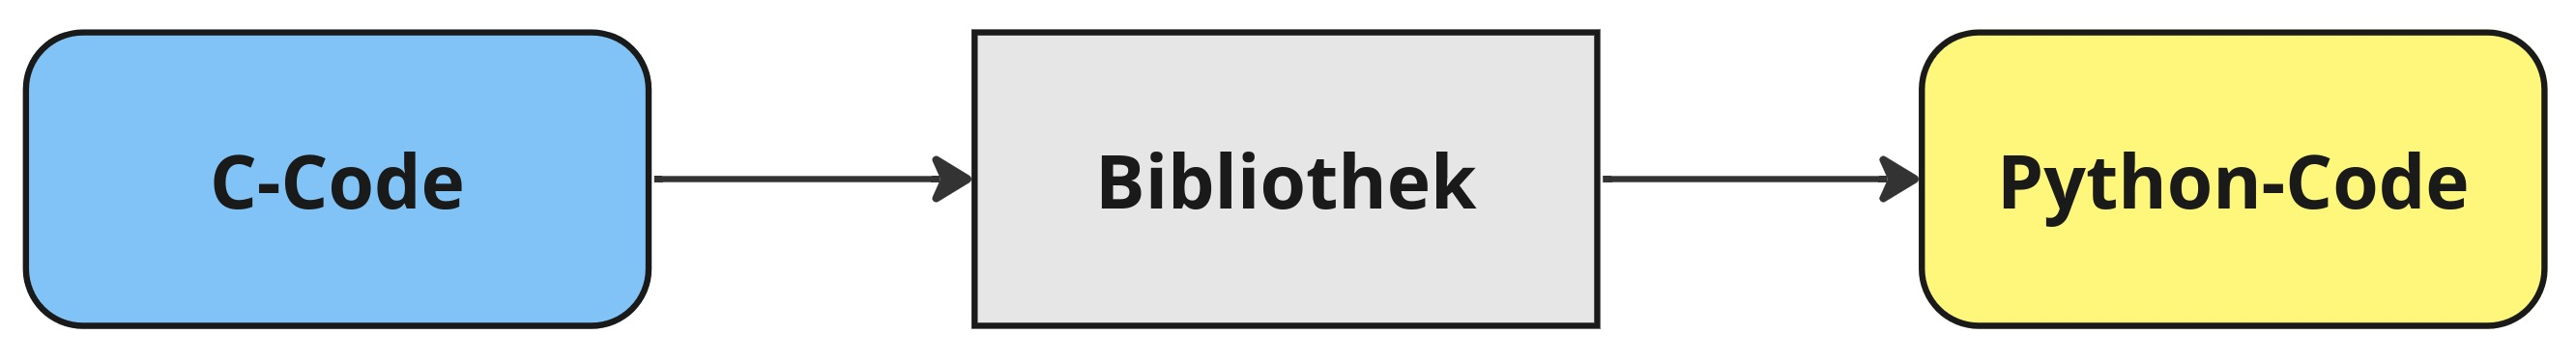
\includegraphics[width=0.7\textwidth]{pipeline.jpg}
    \caption{Pipline C-Code zu Python-Code}
    \label{fig:pipeline}
\end{figure}

Während bei Cython und der C-API jeweils eine Python Bibliothk erstellt wird, wird bei ctypes eine C-Bibliothek erstellt. Das grundlegende Vorgehen ist aber identisch: Das Erstellen einer Bibliothek, die dann in Python importiert wird. 
In Cython und der C-API wird dabei eine C-Datei geschrieben, die dann zum Beispiel über \lstinline{setuptools} zu einer Bibliothek werden.
In ctypes wird C-Code geschrieben, der zu einer C-Bibliothek kompiliert wird. 


\section{Umsetzung der verschiedenen Implementierungen}
Um die Unterschiede zwischen den beiden Programmiersprachen darzustellen, wird ein Programm genutzt, dass eine Textdatei mit 1.000.000 Zahlen ausliest, jede Zahl quadriert, und die Summe der quadrierten Zahlen bildet. 
Die Textdatei wurde mittels bash mit dem Kommando 
\begin{lstlisting}
    i=0; while [ $i -lt 1000000 ]; do echo $(( ($RANDOM%10000)+1 )); i=$((i+1)); done > numbers.txt
\end{lstlisting}
erstellt.     

Das Programm zum Quadrieren und Summieren der Zahlen wurde zuerst jeweils in reinem Python und C geschrieben. 
Für beide Varianten wurde die Komplexität des Codes verglichen und über das linux Kommando \lstinline{time} die Laufzeit gemessen \cite{time}. 
Die Laufzeiten des Python- und C-Codes wurden dann als Benchmark für die Bewertung der Laufzeiten der Imlementierungen in cython, ctypes und der C-API genutzt. 

Sowohl bei der Implementierung in reinem Python, als auch bei der Umsetzung in C wurde versucht, die "best practices" der beiden Sprachen umzusetzen und gleichzeitig den code so effektiv wie möglich zu gestalten. 


\subsection{Reines Python}

In Python ist das Programm wie folgt: 

\lstinputlisting[language=python]{pure_python/main.py}

In dem Code wurde zuerst eine Funktion \lstinline{calculate_sum_of_squares()} definiert, die eine Datei mit 1.000.000 Zahlen öffnet. Jede Zahl aus dieser Datei wird quadriert und zu einer Summe hinzugefügt. Das Ergebnis wird dann in der Konsole ausgegeben. 

Die Ausführungszeit des Python Programms ist wie folgt:

\begin{figure}[H]
    \centering
    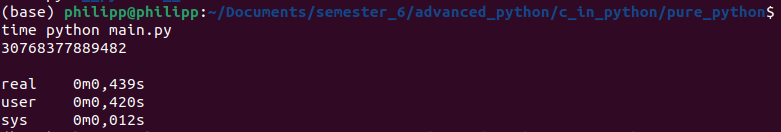
\includegraphics[width=0.9\textwidth]{pure_python/timing_python.png}
    \caption{Timinganalyse Reines Python}
    \label{fig:timing-pure-python}
\end{figure}

In der ersten Zeile der Ausführung wird die Summe der Quadrate ausgegeben, damit die richtige Ausführung des Programms verifiziert werden kann.
Von den drei angezeigten Zeiten ist die real-Zeit die verstrichene Zeit, vom drücken der Enter-Taste bis zum Ende der Ausführung des Programms. Die Zeiten darunter geben an, wie viel Zeit im User-Modus und im Kernel-Modus verbracht wurde.

\subsection{Reines C}

In C ist der Code wie folgt:

\lstinputlisting[language=C]{pure_c/main.c}

In der main wird zu erst die Datei im Lesemodus geöffnet und ein Pointer auf das Dateiobjekt erzeugt. Danach werden die Variablen deklariert, die die Werte beinhalten. Daraufhin wird mit \lstinline{fscanf()} über alle Zeilen der Datei itteriert, die Zahlenwerte ausgelesen, quadriert, und zu der \lstinline{total}-Variable addiert. 
Nachdem alle Zeilen verarbeitet wurden, wird die Datei geschlossen und das Ergebnis ausgegeben. 

Bei Betrachtung des Codes fällt auf, dass im Gegensatz zu Python der Code deutlich komplexer ist. Es muss zu jeder Variable der richtige Datentyp vor der Ausführung bereits festgelegt werden. Selbst bei der Ausführung der \lstinline{printf()}-Funktion muss in der Formatierung darauf geachtet werden, dass der richtige Datentype ausgefählt wird. Außerdem werden pointer benutzt, also Zeiger auf den Speicherort einer Variable. 

Die Performance des reinen C-Codes ist wie folgt:
\begin{figure}[H]
    \centering
    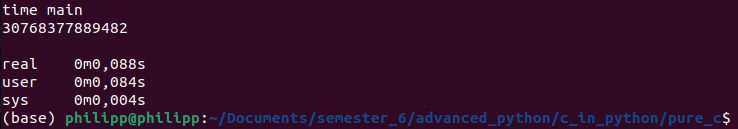
\includegraphics[width=0.9\textwidth]{pure_c/timing_c.png}
    \caption{Timinganalyse Reines C}
    \label{fig:timing-pure-c}
\end{figure}

Hier lässt sich bereits erkennen, dass der C-Code deutlich schneller ist als der Python-Code

\subsection{ctypes}

Um C-Code über ctypes zu nutzen wird der C-Code (fast) ohne Änderungen als .c Datei übernommen. Die einzige Änderung ist, dass aus der main-Funktion eine dedizierte Funktion \lstinline{long int calculate_sum_of_squares(const char *filename)} erstellt wird. Diese Funktion nimmt den Dateinamen als Parameter und gibt ein long int als Rückgabewert zurück. 
Aus diesem Code wird eine Bibliothek erstellt. Der Vorgang ist dabei derselbe wie bei dem Erstellen einer regulären C-Bibliothek.
Das wurde in diesem Fall mittels des gcc-Compilers und dem Kommando \lstinline{gcc -shared -o sum_of_squares_ctypes.so -fPIC sum_of_squares_ctypes.c} erreicht. Die neu erstellte Bibliothek trägt dann den Namen \lstinline{sum_of_squares_ctypes.so} 

In Python wird diese Bibliothek mittels der ctypes-Bibliothek importiert. Hierbei muss nur noch darauf geachtet werden, dass die Datentypen der übergebenen Parameter und der Rückgabewerte definiert werden müssen.

\lstinputlisting[language=Python]{ctypes/main.py}

Über die \lstinline{CDLL()}-Methode von ctypes wird die C-Bibliothek eingebunden. 
Mit \lstinline{lib.calculate_sum_of_squares.argtypes = [ctypes.c_char_p]} wird Python mitgeteilt, welchen Datentyp der übergebene Parameter hat. Mit \lstinline{lib.calculate_sum_of_squares.restype = ctypes.c_long} wird definiert, welcher rückgabewert an python übergeben wird.  
Im Anschluss wird die Funktion wie üblich in Python aufgerufen. 

Die Timinganalyse für die Ctypes-Implementierung ist wie folgt:

\begin{figure}[H]
    \centering
    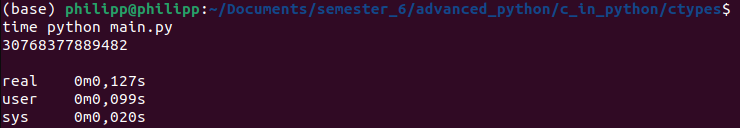
\includegraphics[width=0.9\textwidth]{ctypes/timing_ctypes.png}
    \caption{Timinganalyse Ctypes}
    \label{fig:timing-ctypes}
\end{figure}


Hier lässt sich sehen, dass der Code immer noch deutlich schneller ist als der reine Python-Code, allerdings langsamer als der C-Code.

\subsection{Cython}

Für Cython werden nicht mehr die vorherigen c-Dateien genutzt, sondern es wird eine .pyx Datei erstellt. Diese datei enthält syntaktisch eine Mischung aus C und Pyhon code. In ihr werden die benötigten Datentypen definiert und beschrieben, in welchen C Modulen sie zu finden sind. \cite{cython-syntax}

\lstinputlisting[language=Python]{cython/sum_of_squares_cython.pyx}

Bei Betrachtung der .pyx-Datei lässt sich festestellen, dass die Syntax elemente sowohl von Python als auch von C beinhaltet. 
Datentypen und Funktionen, die nur in C vorhanden sind, werden hier mit dem Schlüsselword \lstinline{cdef} definiert. Das betrifft Datentypen, Pointer, Structs und Funktionen. 

Im oberen Codeblock werden dabei die Funktionen, die aus der \lstinline{stdio}-Bibliothek stammen, definiert um sie für Cython zur Verfügung zu stellen.

Im unteren Codeblock wird die Funktion definiert, die wir zum Aufsummieren der Zahlen nutzen. Die Zeile, in der der Funktionsname definiert wird erinnert dabei syntaktisch stark an python, während der Inhalt der Funktion stark an C angelehnt ist. Hier werden die Funktionen, die im oberen Codeblock bereitgestellt wurden, genutzt.  

Die .pyx Datei muss nun mittles der setuptools von Python in ein Python modul konvertiert werden. Das geschieht über eine setup.py Datei. 
Cython erstellt dabei eine neue, sehr umfangreiche .c Datei, die insgesamt 6511 Zeilen Code enthält und deshalb hier nicht dargestellt werden soll. 
Diese Datei wird dann wie bei ctypes in eine Python bibliothek konvertiert. Im gegensatz zu der ctypes Umsetzung, bei der ein C-Bibliothek erstellt wurde, wird bei cython eine Python Bibliothek erstellt. Dafür werden die \lstinline{setuptools} von Python benutzt.\cite{cython-setup}

\lstinputlisting[language=Python]{cython/setup.py}

Danach kann die neue Bibliothek in Python importiert und wie jede andere Bibliothek genutzt werden.

\lstinputlisting[language=Python]{cython/main.py}

Bezüglich der Performance ergibt sich folgendes:

\begin{figure}[H]
    \centering
    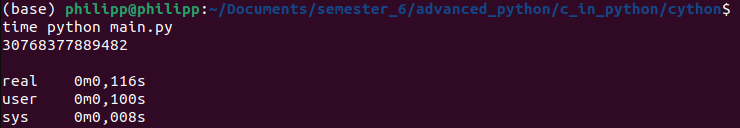
\includegraphics[width=0.9\textwidth]{cython/timing_cython.png}
    \caption{Timinganalyse Cython}
    \label{fig:timing_cython}
\end{figure}


\begin{center}
    
\end{center}

Cython ist demnach schneller als alle bisheringen implementierungen, mit der Ausnahme des reinen C-Codes.



\subsection{Python's C API}

Im C-Code für die nutzung der C-API wird die ursprüngliche C-Funktion übernommen. Darüber hinaus werden diverse Python objekte erzeugt. Dafür wird die \lstinline{"python.h"} Bibliothek includiert. 

\lstinputlisting[language=C]{c_api/sum_of_squares_c_api.c}

Der erste Codeblock ist die gleiche Funktion, die auch schon in der Ctypes Implementierung genutzt wurde. Der Unterschied ist, dass der Code in eine separate Funktion ausgelagert wurde.

In den darauf folgenden Blöcken werden Objekte erzeugt, die für die Umsetzung in Python benötigt werden. 

Die erzeugten Python Objekte sind:
\begin{itemize}
    \item \textbf{PyObject:} Ist eine C Datenstruktur, die als Basistyp für alle möglichen Python objekte eingesetzt wird. Das können Pyhton Datentypen, Objekte oder eingene angelegte Objekte sein. In diesem Fall wird die Funktion
    \lstinline{py_calculate_sum_of_squares(PyObject* self, PyObject* args)} als PyObject angelegt. Der Rückgabewert der Funktion ist ein Pointer zu einem PyObject. Der Übergabewert \lstinline{self} ist aus Python bekannt. \lstinline{args} ist ein pointer auf eine Datenstruktur, die die sonstigen Übergabewerte enthält.
    \lstinline{PyArg_ParseTuple} wird genutzt, um die übergebenen Parameter auszulesen. \\
    In Zeile 25 wird versucht, den Dateinamen aus den Übergabewerten auszulesen und als String in die Variable \lstinline{filename} zu laden. \lstinline{long int result = calculate_sum_of_squares(filename);} ist der Funktionsaufruf in C. Das Ergebnis ist ein long in C und wird in die Variable \lstinline{result} geschrieben. \\
    Zuletzt wird mit der Zeile \lstinline{return PyLong_FromLong (result);} das Ergebnis von einem C long Datentyp in einen Pointer vom Typ \lstinline{PyObject} konvertiert und zurückgegeben. Das PyObject ist in diesem Fall ein Python integer. \cite{c_api_objekte}
    \item \textbf{PyMethodDef:} Ist ein Containerobjekt, das alle einzelnen Funktionen beinhaltet. Die Funktionen werden als Array des Typen \lstinline{PyMethodDef} abgelegt. Für jede Funktion werden Informationen wie der Name der Funktion, ein Pointer zum PyObject hinterlegt, ein Flag zur Beschreibung der Übergabewerte mitgegeben und eine kleine Funktionsbeschreibung hinzugefügt.\\
    Da es in diesem Beispiel nur eine Funktion gibt, wird der Name der Funktion 
    \\\lstinline{calculate_sum_of_squares}, das PyObject \lstinline{py_calculate_sum_of_quares}, das Flag \lstinline{METH_VARARGS}, das aussagt, dass die Funktion ein Tupel als Funktionsparameter erwartet, und der Docstring 'Calculate the sum of squares from a file' hinzugefügt. \cite{c_api_module}
    \item \textbf{PyModuleDef} Ist das Objekt, das das Modul definiert, inklusive des Namens des Moduls und der beinhalteten Funktionen. \lstinline{PyModuleDef_HEAD_INIT} ist ein Makro, das initiallisierungsfunktionen für das Modul ausführt, \lstinline{sum_of_squares_c_api} ist der Name des erstellten Moduls, \lstinline{NULL} ist der Docstring für das Modul, der allerdings optional ist. \lstinline{-1} ist ein Indikator für die Menge des Speichers, der reserviert werden soll. Der Wert -1 deutet an, dass Speicher nicht explizit reservirt wird. Ein positiver integer Wert würde Speicher reservieren. \lstinline{module_methods} ist das Array von Methoden, die im vorherigen Block definiert wurden und in dem Modul enthalten sein sollen. \cite{c_api_module}
    \item \textbf{PyMODINIT\_FUNC} ist eine Funktion die aufgerufen wird, wenn das erstellte Modul in Python importiert wird um die darin definierten Objekte zu initialisieren. \lstinline{PyModule_Create} erstellt dabei das Modulobjekt dynamisch zur Laufzeit aus dem erstellten C Modul. \cite{c_api_init}
\end{itemize}

Der oben beschriebene C-Code wird dann mittels einer \lstinline{"setup.py"} Datei in ein Modul umgewandelt, dass dann in Python importiert werden kann. Die Setup datei ist der aus cython sehr ähnlich, da das Vorgehen beim Erstellen eines Python Moduls grundsätzlich nach dem gleichen Schema verläuft.  

\lstinputlisting[language=Python]{c_api/setup.py}

\lstinputlisting[language=Python]{c_api/main.py}

Interessanterweise wird bei dieser Implementierung der großteil des Implementierungsprozesses in C durchgeführt. Dafür liefert C eine eigene Python Bibliothek. Der Grund dafür ist, dass die API ursprünglich geschrieben wurde, um Python-Code in C ausführen zu können. Dadurch kann man die Stärken von Python nutzen, wie zum Beispiel die Möglichkeit, schnell Prototyp-Code zu erstellen.

\begin{figure}[H]
    \centering
    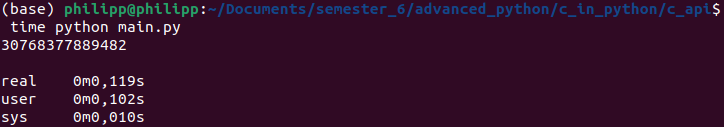
\includegraphics[width=0.9\textwidth]{c_api/timing_c_api.png}
    \caption{Timinganalyse C-API}
    \label{fig:timing_c_api}
\end{figure}

Beim Betrachten der Laufzeit stellt man fest, dass die Implementierung über die C-API nur geringfügig langsamer ist als die Cython-Variante. Der Programmieraufwand ist hingegen höher, da man sich erst mit der \lstinline{python.h}-Bibliothek vertraut machen muss und der resultierende Code etwas umfangreicher ist. 

\section{Laufzeit und Komplexizität}

Nach Auswerten der Laufzeiten mittels des \lstinline{time}-Kommandos in Linux lässt sich folgende Tabelle aufstellen:

\begin{table}[H]
    \centering
    \begin{tabular}{|c|r|c|c|}\hline
         Umsetzung  & Laufzeit & Performancegewinn &  Syntax  \\\hline\hline
         Python     & 0,439s                                &  -        & Einfach \\
         C          & 0,088s                                & 79,95 \% & Mittel \\\hline
         ctypes     & 0,127s                                & 71,07\% & \color{green} Einfach\color{black} \\
         Cython     & \color{green}0,116s\color{black}      & \color{green}73,57\%\color{black} & Mittel \\
         C-API      & 0,119s                                & 72,89\% & Komplex \\\hline
    \end{tabular}    
    \caption{Performance- und Syntaxvergleich}
    \label{tab:performance and syntax comparison}
\end{table}

Die Formel, die zum Ermitteln des Performancegewinns genutzt wurde ist:
\begin{equation}
    \frac{\text{Zeit Python} - \text{Zeit der C-Umsetzung}}{\text{Zeit Python}} \cdot 100
\end{equation}

Reines C ist erwartungsgemäß die performanteste Variante den Beispielcode auszuführen. Von den Python implementierungen ist Cython die Methode, die am meisten Performancegewinne bietet. Die C-API von der Laufzeit her vergleichbar. Die Ctypes-Implementierung bring die geringsten Performancegewinne.

Als Python-Programmierer ist die Syntax des Reinen C-Programms noch relativ übersichtlich. Ctypes bieten von den drei hier untersuchten Implementierungen die einfachste Syntax, da man (sofern ein fertiges C-Programm vorliegt), die Implementinerung direkt in Python vornehmen kann. Die Syntax der Cython implementierung ist etwas gewöhnungsbedürftig, da es sich um einen Hybrid zwischen Python und C handelt. Am Aufwendigsten ist die Implementierung über die C-API da dort einige C-Datenstrukturen angelegt werden müssen, die die benötigten Python Objekte abbilden. 

Hierzu sei aber gesagt, dass die Bewertung der Syntax ein sehr subjektiver Maßstab ist und die Meinung von unterschiedlichen Menschen mit unterschiedlichen Programmiererfahrungen von der hier vorgenommenen Bewertung abweichen kann.

Die Bewertung der Laufzeit ist ebenfalls nicht ohne Einschränkungen hinzunehmen, da sie abhängig von der Komplexität der Programmieraufgabe unterschiedlich ausfallen kann. Zwar ist anzunehmen, dass die Performancegewinne der C-Umsetzungen im Gegensatz zu der reinen Python Implementierung weiterhin deutlich ausfallen werden, die genauen Werte lassen sich durch so ein eingeschränktes Beispiel nur bedingt abbilden.

Eine interessante Nebenbeobachtung aus diesem Projekt war die Umsetzung des Programms in Python mit der Nutzung von Numpy-eigenen Funktionen. Die Idee war, dass die Numpy-Bibliothek aus extrem optimiertem Code besteht und somit vermutlich bessere Laufzeiten als die von mir geschriebenen Implementiereungen von C-Code hat. Interessanterweise war das nicht der Fall. Es zeigte sich, dass nur duch das importieren von Numpy die Laufzeit von $\approx$ 0,283s länger war als bei meinen eigenen Implementierungen (aber immer noch fast doppelt so schnell wie die python implementierung). Ich gehe davon aus, dass der Grund dafür der Umfang der Numpy-Bibliothek ist. Dadurch, dass beim Import von Bibliotheken in Python die Komplette Bibliothek importiert wird (selbst wenn man nur bestimmte funktionen importieren möchte), dauert der Import selbst schon sehr lange. Das konnte ich bestätigen indem ich die Numpy Bibliothek importiert habe, ohne sie zu nutzen. Nur durch den Import hat sich die Performance meines Codes deutlich verschechtert. 
Man kann allerdings davon ausgehen, dass diese Zeit bei komplexeren Programmen nicht stark ins Gewicht fällt.

\section{Zusammenfassung}


In dieser Arbeit wurden drei verschiedenen Arten der Integration von C-Code in Python untersucht und anaylsiert. Namentlich wurden Ctypes, Cython und die C-API betrachtet. Dabei wurde auf die Vor- und Nachteile der verschiedenen Alternativen eingegangen und die Implementierung mit den Umsetzungen in reinem Python beziehungsweise C verglichen. 
Die (einfache) Beispielaufgabe zur Berechnung und Aufsummierung der Quadrate der Zahlen einer Textdatei zeigt, dass cython die beste Performance bietet und dabei immer noch relativ einfach umzusetzen ist. Ctypes bieten den geringsten Performancegewinn, dafür ist die syntax vergleichsweise einfach. Die C-API ist nur geringfügig langsamer als cython, aber dafür deutlich komplexer in der Syntax. 

Bei der Entscheidung, welche Art der C Integration in Python man verfolgen sollte muss man sich Gedanken über die Anforderungen dan die Anwendung machen. Dabei sind die Performance und die Komplexität des Codes von vorrangiger Bedeutung. 

Für code, bei dem die Performance von höchster Bedeutung ist und eine reine C Implementierung nicht in Frage kommt bieten sich sowohl Cython als auch die C-API an. Beide Varianten bieten ähnliche Performancegewinne, unterscheiden sich aber deutlich in der praktischen Umsetzung. Das Maß der Vertrautheit des Programmierers mit den beiden Sprachen kann hier ausschlaggebend für die Entscheidung für eine der beiden Varianten sein.

Im gegensatz zu Cython und der C-API bieten Ctypes die möglichkeit, C-Code schnell und unkompliziert in den eigenen Python Code einzubinden. Die Umsetzung in Python ist für routinierte Python-Entwickler keine Herausforderung und erlaubt es den Vorteil Pythons, schnell zu iterieren und Code-Prototypen zu erstellen.

Die beste Methode für die Integration von C-Code in Python hängt letzten endes von den Anforderungen an die Anwendung ab und den Fähigkeiten des Programmierers. 

Sämtlicher Code dieser Ausarbeitung kann in meinem Github Repository eingesehen werden. \cite{my_github}

\newpage
\printbibliography
\end{document}
